\chapter{Introducción}

Este trabajo se centra en el desarrollo y aplicación de algoritmos cuánticos para la optimización de rutas de entrega y volumen de carga en la empresa Wolf. Utilizando técnicas de computación cuántica, se busca abordar los desafíos específicos relacionados con la eficiencia en la distribución y el aprovechamiento del espacio de carga en una flota de camiones. 

%El primer capítulo es siempre una introducción. En ella debes resumir de forma esquemática pero suficientemente clara lo esencial de cada una de las partes del trabajo. La lectura de este primer capítulo ha de dar una primera idea clara de lo que se pretendía, las conclusiones a las que se ha llegado y del procedimiento seguido.
%Como tal, es uno de los capítulos más importantes de la memoria. Las ideas principales a transmitir son la identificación del problema a tratar, la justificación de su importancia, los objetivos generales (a grandes rasgos) y un adelanto de la contribución que esperas hacer.
%Típicamente una introducción tiene tres apartados: Motivación, Planteamiento del trabajo, Estructura del trabajo. (Texto Normal del menú de estilos.)
%(Ejemplo de nota al pie\footnote{Ejemplo de nota al pie.}.)

\section{Motivación}

    El transporte y la logística son vitales para la economía global, pero enfrentan problemas significativos relacionados con la optimización de rutas y la carga de vehículos. Las soluciones actuales son a menudo ineficientes, llevando a un uso subóptimo de recursos, aumento de costos y tiempo de entrega. Este trabajo identifica y aborda estas ineficiencias utilizando algoritmos cuánticos, que prometen una capacidad superior para manejar la complejidad y dinamismo de tales sistemas.
    La importancia de optimizar rutas de entrega y carga se magnifica en contextos de alta demanda y diversidad geográfica, como lo es el caso de la empresa Wolf. Los desafíos incluyen la gestión eficiente de múltiples puntos de recolección y distribución, la variabilidad en el tamaño y volumen de los paquetes, y restricciones temporales estrictas. La computación cuántica ofrece un enfoque prometedor para superar estos retos, lo que podría resultar en una significativa reducción de costos operativos y mejora en la eficiencia del servicio.


%Cuál es el problema que quieres tratar? ¿Cuáles crees que son las causas? ¿Por qué es relevante el problema?

%A continuación, se indica con un ejemplo cómo deben introducirse los títulos y las fuentes en Tablas y Figuras.

%\begin{table}[t]
%	\begin{center}
%	\caption{Ejemplo de tabla con sus principales elementos.}
%	\label{tab:1}
%	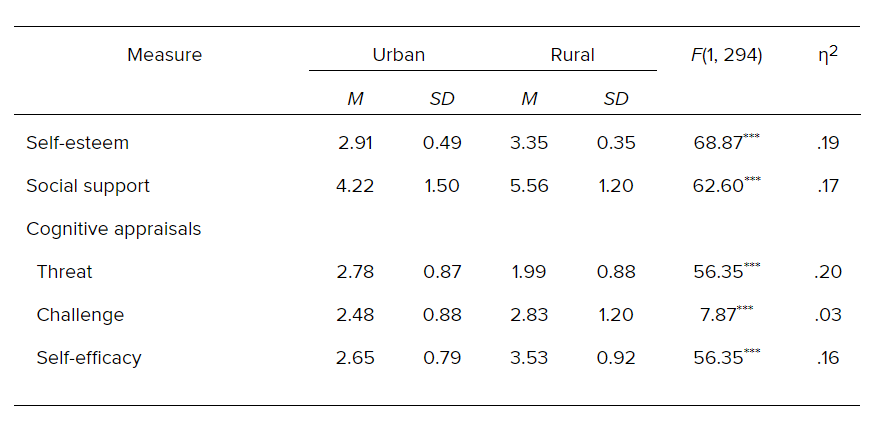
\includegraphics[width=4.90737in,height=2.42708in]{tabla}
%	\small Fuente: American Psychological Association, 2020e.
%	\end{center}
%\end{table}

%\begin{figure}[H]
%	\begin{center}
%		\caption{Ejemplo de figura realizada para nuestro trabajo.}
%		\label{fig:1}
%		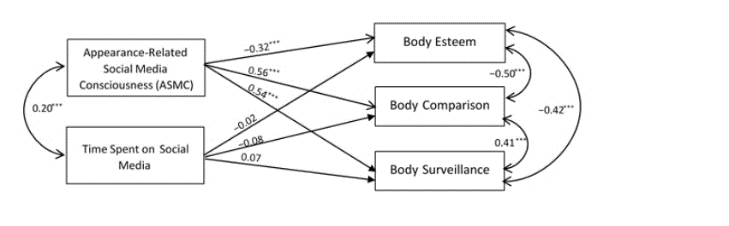
\includegraphics[width=4.90737in,height=2.42708in]{figura}
%%		\small Fuente: American Psychological Association, 2020f.
%	\end{center}
%\end{figure}

\section{Planteamiento del trabajo}

    Este estudio se centra en el desarrollo y evaluación de algoritmos cuánticos diseñados para optimizar las rutas de entrega y la carga de camiones para la empresa Wolf. Se analizarán y compararán estos algoritmos con métodos clásicos de optimización para determinar su viabilidad y eficacia. Dividiremos el probleam en tres partes específicos:

    \begin{itemize}
    \item Optimización de rutas: Desarrollar un algoritmo que mejore la eficiencia de las rutas de entrega, teniendo en cuenta la ubicación geográfica de los puntos de distribución, el tamaño y volumen de los paquetes, y los intervalos de tiempo de entrega.
    
    \item Planificación de itinerarios: Crear un sistema que detalle el tiempo estimado de llegada para cada vehículo a todos los puntos de distribución.
    
    \item Optimización de la carga: Mejorar el proceso de carga de los vehículos, ordenando los paquetes de manera que se maximice el uso del espacio disponible y se optimice la eficiencia del transporte.
    
    La investigación evaluará la aplicabilidad de varios algoritmos cuánticos, incluyendo el recocido cuántico y el algoritmo de Grover, y utilizará plataformas como IBM Quantum, D-Wave y Rigetti.
    \end{itemize}

%¿Cómo se podría solucionar el problema? ¿Qué es lo que se propone? Aquí describes tu objetivo en términos generales. 

\section{Estructura de la memoria}

    Este trabajo estará organizado en los siguientes capítulos para abordar de manera sistemática el problema de investigación:

    \textbf{Introducción:} Presentación del problema, justificación y objetivos del estudio.
    Fundamentos Teóricos: Explicación de los conceptos básicos de la mecánica cuántica y la computación cuántica necesarios para entender los algoritmos utilizados.
    
    \textbf{Metodología:} Detalle de las técnicas y herramientas cuánticas seleccionadas, así como la metodología de comparación con sistemas clásicos.
    Desarrollo de Algoritmos y Simulaciones: Diseño de los algoritmos cuánticos y realización de simulaciones para evaluar su rendimiento.
    
    \textbf{Resultados y Análisis:} Presentación y análisis de los resultados obtenidos, comparando las soluciones cuánticas con las clásicas.
    
   \textbf{ Conclusiones y Recomendaciones:} Síntesis de los hallazgos y sugerencias para futuras investigaciones o aplicaciones prácticas. 

%Aquí describes brevemente lo que vas a contar en cada uno de los capítulos siguientes.